\documentclass[12pt]{article}

\usepackage{pst-all}
\usepackage{demo}

\let\orgheader\adviheader
\def\adviheader{\orgheader\advibg{image=adviback.ppm}}

%Didier's flashy macro
\def \flash #1{\let \do\leflash \do #1\relax}
\def \leflash #1{\ifx #1\relax \def \do{}\else \def \do {#1\adviwait[1]\leflash}\fi \do}

\advibg[global]{image=adviback.ppm}
\begin{document}
\newpage

\subsection* {Active dvi is:}

A {\bf dvi} previewer (based on {\tt mldvi} by Alexandre Miquel)

\bigskip

\noindent
\advitransbox{wipe,from=left}{%
\begin{minipage}{\textwidth}
\begin {itemize}
\item[+] dvips
  \textcolor{c1}{c}%
  \textcolor{c2}{o}%
  \textcolor{c3}{l}%
  \textcolor{c4}{o}%
  \textcolor{c5}{u}%
  \textcolor{c6}{r}
  extension (by Alexandre Miquel)
\item[+] bitmap inclusion with cache (by Jun Furuse)
\item[+] GPIC specials (by Xavier Leroy)
\item[+] Postscript specials (by Didier R{\'{e}}my)
\item[+] hyperrefs (by Didier R{\'{e}}my)
\item[+] active anchors with annotated texts (by Didier R{\'{e}}my)
\item[+] animations and transitions (Jun Furuse and Didier R\'emy)
\item[+] swallowed applications (Jun Furuse and Pierre Weis)
\item[+] and other gadgets...
\end {itemize}
\end{minipage}}

\newpage
\advitransition{wipe}

\subsection*{Presentation macros}
\noindent
\verb|\adviwait|\\
\verb|\advirecord{|{\em text\ }\verb|}|, 
\verb|\adviplay|\\
\verb|\begin{advirecording}|
{\em text}
\verb|\end{advirecording}|

\bigskip

\noindent
Press any key to launch  the demo:
\adviwait

\advitransition{none} % we must reset the transition
\noindent
\verb+\adviwait[+{\em time}\verb+]+ counts down for you:
3\ldots\adviwait[1]2\ldots\adviwait[1]1\ldots\adviwait[1]\textcolor{red}{GO!}

\vfill

\noindent
\begin{tabular}{l}
\advirecord{H}{Hamlet}: Do you see yonder cloud that's almost in shape of a \advirecord{C}{\rnode{CN1}{camel}}?\\
\advirecord{P}{Plonius}: By th'mass, and 'tis like a \advirecord{C}{\rnode{CN2}{camel}}, indeed\\
\advirecord{H}{Hamlet}: Methinks it is like a \advirecord{W}{\rnode{CN3}{weasel}}\\
\advirecord{P}{Plonius}: It is back'd like a \advirecord{W}{\rnode{CN4}{weasel}}\\
\advirecord{H}{Hamlet}: Or like a \advirecord{W2}{\rnode{CN5}{whale}}?\\
\advirecord{P}{Plonius}: Very like a \advirecord{W2}{\rnode{CN6}{whale}}.
\end{tabular}\\
\noindent
{\small \hfill (\advirecord{H}{Hamlet}  by William Shakespeare, Act III, scene 3.)}

\begin{enumerate}
\item Who are they ? \advirecord{H}{Hamlet} and \advirecord{P}{Plonius}.
\advirecord{Q2}{\item What do they say ? \advirecord{C}{Camel}, \advirecord{W}{weasel} and \advirecord{W2}{whale}.}
\advirecord{Q3}{\item And what do they actually see ? \advirecord{C2}{Of course, \rnode{CN0}{\textcolor{red}{CAML!}}}}
\end{enumerate}

\adviwait
\adviplay[red]{H}
\adviwait
\adviplay[black]{H}
\adviplay[red]{P}
\adviwait
\adviplay[black]{P}
\adviplay{Q2}
\adviwait
\adviplay[red]{C}
\adviwait
\adviplay[black]{C}
\adviplay[red]{W}
\adviwait
\adviplay[black]{W}
\adviplay[red]{W2}
\adviwait
\adviplay[black]{W2}
\adviplay{Q3}
\adviwait
\adviplay{C2}
\nccurve[linecolor=red,linewidth=3pt,angleA=0,angleB=280]{->}{CN0}{CN1}
\nccurve[linecolor=red,linewidth=3pt,angleA=0,angleB=350]{->}{CN0}{CN2}
\nccurve[linecolor=red,linewidth=3pt,angleA=0,angleB=350]{->}{CN0}{CN3}
\nccurve[linecolor=red,linewidth=3pt,angleA=0,angleB=355]{->}{CN0}{CN4}
\nccurve[linecolor=red,linewidth=3pt,angleA=0,angleB=0]{->}{CN0}{CN5}
\nccurve[linecolor=red,linewidth=3pt,angleA=0,angleB=0]{->}{CN0}{CN6}
\vfill

\vfill

\newpage
\advitransition{wipe}

\subsection*{EPS Bitmap inclusion}
\begin{center}
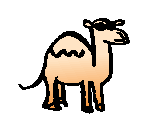
\includegraphics[width=0.15\textwidth,height=0.15\textwidth]{../tex/caml.eps}
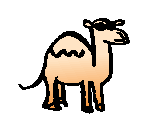
\includegraphics[width=0.3\textwidth,height=0.15\textwidth]{../tex/caml.eps}  
\end{center}

\subsection*{GPIC: Pictures for \TeX}

\def\showgraph{%
  \par\medskip\centerline{\raise 1em\box\graph}\bigskip\noindent\ignorespaces}
\expandafter\ifx\csname graph\endcsname\relax \csname newbox\endcsname\graph\fi
\expandafter\ifx\csname graphtemp\endcsname\relax \csname newdimen\endcsname\graphtemp\fi
\setbox\graph=\vtop{\vskip 0pt\hbox{%
    \special{pn 8}%
    \special{ar 1050 1350 900 900 0 6.28319}%
    \graphtemp=.5ex\advance\graphtemp by 1.440in
    \rlap{\kern 0.960in\lower\graphtemp\hbox to 0pt{\hss O\hss}}%
    \graphtemp=.5ex\advance\graphtemp by 2.550in
    \rlap{\kern 1.050in\lower\graphtemp\hbox to 0pt{\hss The trigonometric circle\hss}}%
    \graphtemp=\baselineskip\multiply\graphtemp by 1\divide\graphtemp by 2
    \advance\graphtemp by .5ex\advance\graphtemp by 1.350in
    \rlap{\kern 1.950in\lower\graphtemp\hbox to 0pt{~1\hss}}%
    \graphtemp=\baselineskip\multiply\graphtemp by -1\divide\graphtemp by 2
    \advance\graphtemp by .5ex\advance\graphtemp by 0.450in
    \rlap{\kern 1.050in\lower\graphtemp\hbox to 0pt{\hss 1~}}%
    \special{pa 0 1350}%
    \special{pa 2400 1350}%
    \special{fp}%
    \special{sh 1.000}%
    \special{pa 2300 1325}%
    \special{pa 2400 1350}%
    \special{pa 2300 1375}%
    \special{pa 2300 1325}%
    \special{fp}%
    \graphtemp=\baselineskip\multiply\graphtemp by 1\divide\graphtemp by 2
    \advance\graphtemp by .5ex\advance\graphtemp by 1.350in
    \rlap{\kern 2.400in\lower\graphtemp\hbox to 0pt{\hss $x$}}%
    \special{pa 1050 2400}%
    \special{pa 1050 0}%
    \special{fp}%
    \special{sh 1.000}%
    \special{pa 1025 100}%
    \special{pa 1050 0}%
    \special{pa 1075 100}%
    \special{pa 1025 100}%
    \special{fp}%
    \graphtemp=.5ex\advance\graphtemp by 0.000in
    \rlap{\kern 1.050in\lower\graphtemp\hbox to 0pt{\hss $y$~}}%
    \special{ar 1282 1319 250 250 -0.886486 0.125474}%
    \special{sh 1.000}%
    \special{pa 1502 1208}%
    \special{pa 1440 1125}%
    \special{pa 1533 1169}%
    \special{pa 1502 1208}%
    \special{fp}%
    \graphtemp=\baselineskip\multiply\graphtemp by -1\divide\graphtemp by 2
    \advance\graphtemp by .5ex\advance\graphtemp by 1.319in
    \rlap{\kern 1.532in\lower\graphtemp\hbox to 0pt{~$\theta$\hss}}%
    \special{pa 1050 1350}%
    \special{pa 1829 900}%
    \special{fp}%
    \graphtemp=.5ex\advance\graphtemp by 0.800in
    \rlap{\kern 1.929in\lower\graphtemp\hbox to 0pt{\hss $M$\hss}}%
    \special{pa 1829 900}%
    \special{pa 1050 900}%
    \special{fp}%
    \special{sh 1.000}%
    \special{pa 1150 925}%
    \special{pa 1050 900}%
    \special{pa 1150 875}%
    \special{pa 1150 925}%
    \special{fp}%
    \graphtemp=.5ex\advance\graphtemp by 1.125in
    \rlap{\kern 0.810in\lower\graphtemp\hbox to 0pt{\hss $\sin\left(\theta\right)\left\{\begin{array}{c} \\ \\ \end{array}\right.$\hss}}%
    \special{pa 1829 900}%
    \special{pa 1829 1350}%
    \special{fp}%
    \special{sh 1.000}%
    \special{pa 1854 1250}%
    \special{pa 1829 1350}%
    \special{pa 1804 1250}%
    \special{pa 1854 1250}%
    \special{fp}%
    \graphtemp=.5ex\advance\graphtemp by 1.350in
    \rlap{\kern 1.829in\lower\graphtemp\hbox to 0pt{\hss $\underbrace{\hspace*{1.95cm}}_{\displaystyle\cos~\left(\theta\right)~}$}}%
    \hbox{\vrule depth2.550in width0pt height 0pt}%
    \kern 2.400in
  }%
}%
\showgraph


\subsection*{PsTricks macros}
\begin{center}
\begin{pspicture}(0.8\textwidth,0.13\textheight)
\psset{linestyle=none,fillstyle=solid}
\rput(0.1\textwidth,0.0\textheight){\ovalnode[fillcolor=lightred]{A}{A}}
\rput(0.2\textwidth,0.1\textheight){\ovalnode[fillcolor=lightgreen]{B}{B}}
\rput(0.4\textwidth,0.02\textheight){\ovalnode[fillcolor=lightblue]{C}{C}}
\rput(0.5\textwidth,0.125\textheight){\ovalnode[fillcolor=yellow]{D}{D}}
\rput(0.7\textwidth,0.05\textheight){\ovalnode[fillcolor=cyan]{E}{E}}
\psset{linestyle=solid,fillstyle=none}
\ncline{->}{A}{B}
\ncline{->}{B}{C}
\ncline{->}{C}{D}
\ncline{->}{D}{E}
\psset{linestyle=dashed}
\ncdiag[linearc=.5,angleA=10,angleB=190,nodesep=2pt]{->}{A}{D}
\nccircle[angleA=180,nodesep=2pt,linearc=.2]{<-}{C}{20pt}
\end{pspicture}
\end{center}

\newpage
\advitransition{slide,from=top}

\subsection*{Embedded applications}
\verb|\adviembed{|%
{\em width}%
\verb|}{|%
{\em height}%
\verb|}{|%
{\em command}%
\verb|}|\\[2mm]

\noindent
\begin{tabular}{ll}
  \begin{minipage}[t]{0.4\textwidth}
    {\bf Simple clock}\\[2mm]
    \adviembed[persistent=clock,width=5cm,height=0.71cm]{wish ./watch -geometry !g -use !p}

    \vspace{2cm}

    {\bf Animation}\\[2mm]
    \adviembed[width=2cm,height=2cm]{animate -geometry !g! -window !p mmm.anim.gif}

    \vspace{2cm}


    {\bf Music}\\[1mm]
    Click the following buttons!
\advirecord{play}{\adviembed[name=mpg123,width=1mm,height=1mm]{mpg123 -q music.mp3}}
\advirecord {stop}{\advikillembed {mpg123}}
\advianchor[click]{play}{Play}
\advianchor[click]{stop}{Stop}
   \end{minipage}
&

  \begin{minipage}[t]{0.5\textwidth}
    {\bf Puzzle}\\[2mm]
    \adviembed[persistent=taquin,width=7.5cm,height=11cm]{./taquin.sh -geometry !g -use !p dojoji.gif}
  \end{minipage}
\end{tabular}

\newpage
\advitransition{slide,from=left}

\subsection*{WM managed applications}
\verb|\adviembed[width=|%
{\em width}%
\verb|,height=|%
{\em height}%
\verb|]{|%
{\em command}%
\verb|}|

\bigskip

Their position may be incorrect.
Change your WM configulation so that it does not
remember the window positions.

\vfill

\noindent
{\bf Eyes}\\[2mm]
\adviembed[width=3cm,height=3cm]{xeyes -bw 0 -shape -geometry !g}

\vfill

\noindent
{\bf O'Caml toplevel}\\[2mm]
\adviembed[width=10cm,height=2cm]{xterm -geometry 50x5+!x+!y -e ocaml}

\vfill

\vfill

\vfill



\end{document}
